\documentclass[%
 reprint,
%superscriptaddress,
%groupedaddress,
%unsortedaddress,
%runinaddress,
%frontmatterverbose, 
%preprint,
%showpacs,preprintnumbers,
%nofootinbib,
%nobibnotes,
%bibnotes,
 amsmath,amssymb,
 aps,
%pra,
%prb,
%rmp,
%prstab,
%prstper,
%floatfix,
]{revtex4-1}

\usepackage{graphicx}% Include figure files
\usepackage{dcolumn}% Align table columns on decimal point
\usepackage{bm}% bold math
\usepackage{comment}
\usepackage{float}
%\usepackage{hyperref}% add hypertext capabilities
%\usepackage[mathlines]{lineno}% Enable numbering of text and display math
%\linenumbers\relax % Commence numbering lines

%\usepackage[showframe,%Uncomment any one of the following lines to test 
%%scale=0.7, marginratio={1:1, 2:3}, ignoreall,% default settings
%%text={7in,10in},centering,
%%margin=1.5in,
%%total={6.5in,8.75in}, top=1.2in, left=0.9in, includefoot,
%%height=10in,a5paper,hmargin={3cm,0.8in},
%]{geometry}

\begin{document}

%\preprint{APS/123-QED}

\title{FP2 - W and Z boson decay}% Force line breaks with \\


\author{Marco Canteri}

\author{Johannes Willi}

\date{\today}% It is always \today, today,
             %  but any date may be explicitly specified

\begin{abstract}
In this work we have analysed several events from the detector ATLAS in order to identify and study two bosons: W boson and Z boson. The study is divided in three parts: first of all
we looked at 40 events and found a ratio between W and Z decays of $W/Z = 6 \pm 3.5$; second we tried to reconstruct the proton structure starting from 100 events of W boson decays; in the third part we focused on Z boson decays and we obtained a mass of Z of $\pm $ Gev, a particle candidate for Higgs boson of mass $\pm$, and a possible Z$'$ boson of mass $\pm$ Gev.
\end{abstract}
\maketitle

%\tableofcontents

\section{\label{sec:level1}Introduction}
In Geneva, 100 meters under ground, protons are collided inside a circumference of 27 kilometers. The ATLAS detectors is build to detect particles created from these collisions.
ATLAS is composed manly by three parts: a tracking chamber that can detect charged particle and can give information about charge, momentum, energy; electromagnetic and hadronic calorimeter where photons, electrons, positrons and hadronic particles leave a deposit of energy; and a muon chamber for detecting muons, which don't stop inside the calorimeters. In addition it is possible to indirectly observe neutrinos by computing the missing transverse momentum. The main purpose of this work is to study the gauge particles for weak interaction: Z boson and W boson. Due to the short life of these bosons (around $10^{-25}$ s), the main possibility of study these particles is by means of decay products. Indeed W and Z bosons can decay in leptons or quarks that have a longer life. We didn't study every possible decay channel, but instead we focused on those which have detectable particles as decay products. For example a W boson can decay in a pair of lepton and neutrino or in a pair of up-down quarks. The easiest particles of W decay to identify in ATLAS are electrons and muons and the respective antiparticles, so the channel we focused on are
\[W^- \to e^- + \overline{\nu}_e \qquad W^- \to \mu^- + \overline{\nu}_\mu\]
\[W^+ \to e^+ + \nu_e \qquad W^+ \to \mu^+ + \nu_\mu. \]
The Z boson decay in a pair of lepton and antilepton 10\% of cases, 20\% in neutrino and antineutrino and 70\% in quark antiquark pairs. Again, since we are dealing with ATLAS events, we search for the easiest decay channels that we can be see in our detector. Those decays are
\[Z \to e^+ + e^- \qquad Z \to \mu^+ + \mu^-.\]
Furthermore, among all the events we also searched evidence of Higgs boson decays through these decay channels
\[H \to \gamma + \gamma \quad H \to Z+ Z \qquad H \to W^+ + W^-.\]
\\


\section{W/Z events ratio}
We used HYPATIA in order to analyse $N=40$ simulated events, in table \ref{tab:table1} we reported the number of events that we observed in our data.
The ratio between observed decays of W and Z boson is $ N_W/N_Z = 6\pm 3.5$, where the error is calculated through the error propagation of $N_W/N_Z$. As errors of $N_W$ and $N_Z$ we used the standard deviation of the multinomial distribution
\[\sigma_W^2 =  N_W\left(1-\frac{N_W}{N}\right) \qquad \sigma_Z^2 =  N_Z\left(1-\frac{N_Z}{N}\right).\]

\begin{table}[h]
\begin{ruledtabular}
\begin{tabular}{cccccc}
 $W\to e\nu$ & $W\to \mu\nu$ & $Z\to ee$ & $Z\to \mu\mu$ & $H\to 4l$ & Background \\
\hline
8 & 10 & 1 & 2 & 0 & 19
\end{tabular}
\end{ruledtabular}
\caption{\label{tab:table1}Number of events identified in our data. We made no distinction between particles and their antiparticles. Here $l$ means any lepton}
\end{table}

\section{Proton structure}

\begin{table*}
\begin{ruledtabular}
\begin{tabular}{cccccc}
 $\text{W}^+\to e^+ + \nu_e$ & $\text{W}^-\to e^- + \bar{\nu}_e$ & $\text{W}^+\to \mu^+ + \nu_\mu$ & $\text{W}^-\to \mu^- + \bar{\nu}_\mu$ & $\text{H}\to \text{W}^++\text{W}^-  $& Background \\
\hline
21 & 9 & 25 & 10 & 3 & 32
\end{tabular}
\end{ruledtabular}
\caption{\label{tab:table2}Number of events identified in our data}
\end{table*}
We analysed 100 events with the software MINERVA searching for W boson decays. In order to understand the proton structure we needed to distinguish between $\text{W}^+$ boson and $\text{W}^-$ boson, in fact a proton is composed by up and down quarks. Therefore, a $\text{W}^+$ is produced by a quark up and a $\text{W}^-$ by a quark down. Hence is possible to determine the ratio between quark up and quark down inside a proton by calculating the ratio between a production of a $\text{W}^+$ boson and a $\text{W}^+-$ boson via gluon quark interaction. As can be seen in our date from table \ref{tab:table2} the ratio between $\text{W}^+$ and $\text{W}^-$ is $W_+/W_- = 2.38 \pm 0.62$, which is compatible with [] $1.52 \pm 0.07$. The error is calculated by propagation on the ratio and the error of very event is the standard deviation of the Poisson distribution, such as in the previous section. We only need W boson that are product of an interaction between quark and gluon. It is possible to calculate those events by knowing the probability of having a gluon-gluon interaction versus a gluon-quark interaction. Let $R_{\pm}$ be the number of $\text{W}^\pm$ decay as product of quark-gluon interacion, so
\[\frac{W_+}{W_-} = \frac{R_+ + a}{R_- + b},\]
where $a$ and $b$ are respectively the number of $\text{W}^\pm$ due to gluon-gluon interaction. From theory it is possible to derive that $a = b = N/6$, where $N$ is the total number of events. Therefore, it easy to calculate $R_+ = W_+ -a$ and $R_- = W_- -b$. In our case we obtained $R_+/R_- = 4.16 \pm 2.26$.
\section{Z decays and mass determination}
\begin{minipage}{\textwidth}
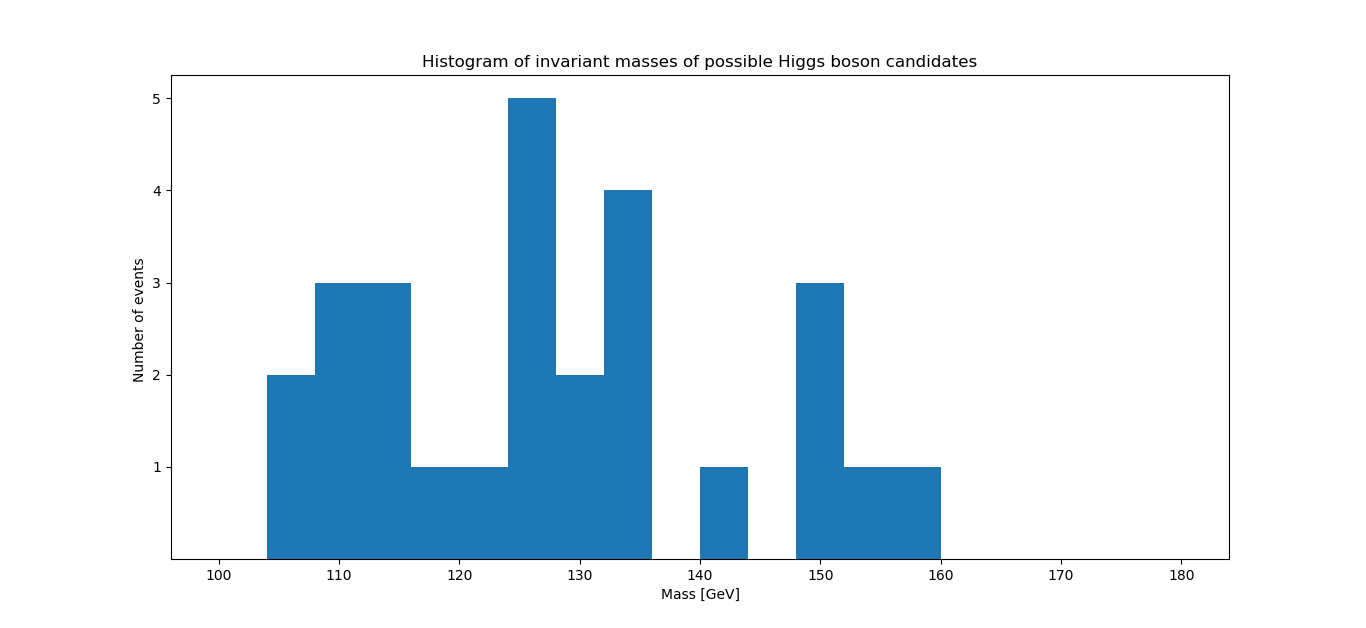
\includegraphics[width=\textwidth]{img/higgs}
%\caption{Histogram for Higgs boson candidates}
\end{minipage}

In order to estimate the mass of the Z boson we analysed 100 events with the software HYPATIA and did the same for the Higgs boson. After the identification of the events, i.e. $Z \to l\bar{l}$, $H\to \gamma\gamma$, and $H\to ZZ\to4l$, we used the Invariant Mass tool to evaluate the mass of the particle decayed. In figure () we plotted an histogram for all the events of possible Higgs candidates. The mean value of the mass is $127.8\pm 3.0$ GeV, where the error is the standard deviation of the data divided by the square root of the number of data. The result is compatible with the literature value \cite{masshiggs} of  $125.09\pm 0.32$ GeV.

For the Z boson the data are in figure (), as can be seen, there is a peak near 90 GeV, which it is what we expected, but there are also some data in the order of 1000 GeV. These data could be candidates for a possible Z$'$ boson. The estimated mass of the Z boson is $90.0\pm1.3$ GeV, while for the possible Z$'$ boson is $1150\pm85$ GeV, with error calculated as for the Higgs boson. The Z mass is compatible with the real val ue \cite{Zmass} $91.1876 \pm 0.0021$ GeV. Another estimation for the Z mass can be obtained with a Lorentz fit over the histogram, this is depicted in figure (). The fit is done with the function
\[f(x) = \frac{1}{\pi}\frac{\Gamma}{(x-m)^2+\Gamma^2}\]
where $m$ and $\Gamma$ are two parameters to be determined with the fit and they are the x-value for the peak and the half width half maximum of the distribution. The best fit gave us $m = 90.7$ GeV and $\Gamma = 2.1$ GeV.
%\begin{figure}[h]
%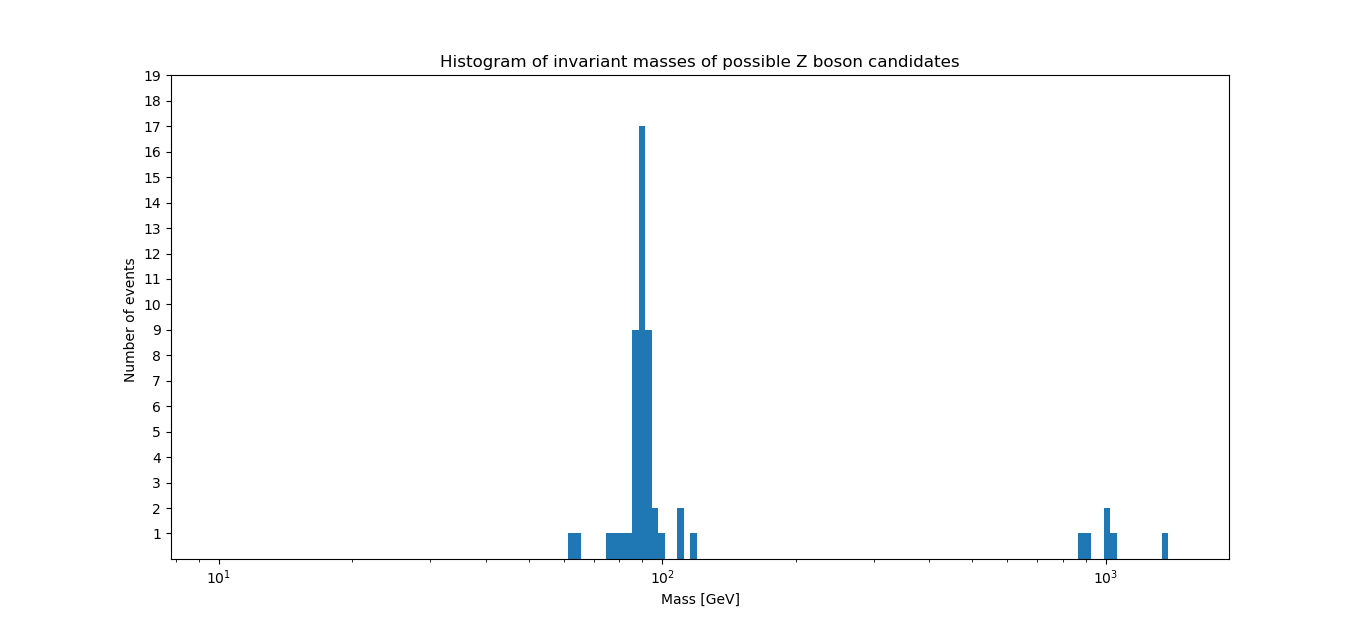
\includegraphics[width =.5\textwidth]{img/Zboson}% Here is how to import EPS art
%\end{figure}
%\begin{figure}[h]
%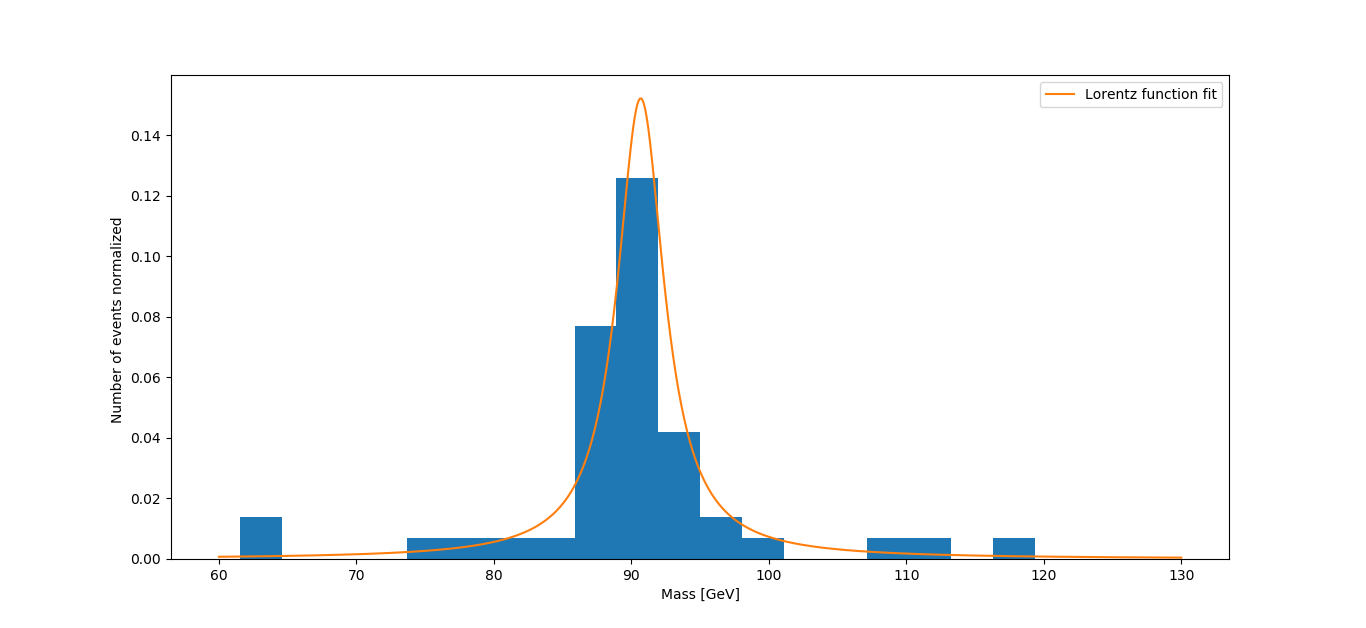
\includegraphics[width =.5\textwidth]{img/Zfit}% Here is how to import EPS art
%\end{figure}
\section{Bibliography}
\begin{thebibliography}{99}

  \bibitem{masshiggs}
    G. Aad et al. (ATLAS Collaboration, CMS Collaboration) Phys. Rev. Lett. {\bf 114}, 191803

  \bibitem{Zmass}
   J. Beringer et al. (Particle Data Group), PR D86, 010001 (2012)

\end{thebibliography}

\end{document}

